%% 
%% Copyright 2007-2020 Elsevier Ltd
%% 
%% This file is part of the 'Elsarticle Bundle'.
%% ---------------------------------------------
%% 
%% It may be distributed under the conditions of the LaTeX Project Public
%% License, either version 1.2 of this license or (at your option) any
%% later version.  The latest version of this license is in
%%    http://www.latex-project.org/lppl.txt
%% and version 1.2 or later is part of all distributions of LaTeX
%% version 1999/12/01 or later.
%% 
%% The list of all files belonging to the 'Elsarticle Bundle' is
%% given in the file `manifest.txt'.
%% 
%% Template article for Elsevier's document class `elsarticle'
%% with harvard style bibliographic references

%LTeX: language=en-GB
\documentclass[preprint,12pt]{elsarticle}

%% Use the option review to obtain double line spacing
%% \documentclass[preprint,review,12pt]{elsarticle}

%% Use the options 1p,twocolumn; 3p; 3p,twocolumn; 5p; or 5p,twocolumn
%% for a journal layout:
%% \documentclass[final,1p,times]{elsarticle}
%% \documentclass[final,1p,times,twocolumn]{elsarticle}
%% \documentclass[final,3p,times]{elsarticle}
%% \documentclass[final,3p,times,twocolumn]{elsarticle}
%% \documentclass[final,5p,times]{elsarticle}
%% \documentclass[final,5p,times,twocolumn]{elsarticle}

%% For including figures, graphicx.sty has been loaded in
%% elsarticle.cls. If you prefer to use the old commands
%% please give \usepackage{epsfig}

\usepackage{graphicx}
\usepackage{caption}
\usepackage{subcaption}
\usepackage{amsmath}
\usepackage{color,soul} % text highlighting
\usepackage[table]{xcolor}
\usepackage{array}
\usepackage{tikz,pgfplots} % for tikz pictures
\usepackage{tabularx}
\usepackage[]{mdframed}
\usepackage{float}
\usepackage{hyperref} % allows _ in urls
% \usepackage{placeins}
\usetikzlibrary{bayesnet} % also need this for my tikz picture...
\newcolumntype{?}[1]{!{\vrule width #1}}

%% The amssymb package provides various useful mathematical symbols
\usepackage{amssymb}
%% The amsthm package provides extended theorem environments
%% \usepackage{amsthm}

%% The lineno packages adds line numbers. Start line numbering with
%% \begin{linenumbers}, end it with \end{linenumbers}. Or switch it on
%% for the whole article with \linenumbers.
%% \usepackage{lineno}

\journal{Mechanical Systems and Signal Processing}

\begin{document}

\begin{frontmatter}

%% Title, authors and addresses

%% use the tnoteref command within \title for footnotes;
%% use the tnotetext command for theassociated footnote;
%% use the fnref command within \author or \address for footnotes;
%% use the fntext command for theassociated footnote;
%% use the corref command within \author for corresponding author footnotes;
%% use the cortext command for theassociated footnote;
%% use the ead command for the email address,
%% and the form \ead[url] for the home page:
%% \title{Title\tnoteref{label1}}
%% \tnotetext[label1]{}
%% \author{Name\corref{cor1}\fnref{label2}}
%% \ead{email address}
%% \ead[url]{home page}
%% \fntext[label2]{}
%% \cortext[cor1]{}
%% \affiliation{organization={},
%%             addressline={},
%%             city={},
%%             postcode={},
%%             state={},
%%             country={}}
%% \fntext[label3]{}

\title{Inter-turbine Modelling of Wind-Farm Power using Multi-task Learning}

%% use optional labels to link authors explicitly to addresses:
%% \author[label1,label2]{}
%% \affiliation[label1]{organization={},
%%             addressline={},
%%             city={},
%%             postcode={},
%%             state={},
%%             country={}}
%%
%% \affiliation[label2]{organization={},
%%             addressline={},
%%             city={},
%%             postcode={},
%%             state={},
%%             country={}}

% \def\correspondingauthor{\footnote{Corresponding author. 
% E-mail address: sbrealy1@gmail.com (S.M. Brealy).}}

\author[inst1]{Simon M.\ Brealy\corref{cor1}}
\ead{sbrealy1@gmail.com}

\affiliation[inst1]{organization={Dynamics Research Group}, %Department and Organization
            addressline={Department of Mechanical Engineering, The University of Sheffield, Mappin Street}, 
            city={Sheffield},
            postcode={S1 3JD}, 
            % state={},
            country={UK}}


\author[inst2]{Lawrence A.\ Bull}


\affiliation[inst2]{organization={School of Mathematics and Statistics}, %Department and Organization
            addressline={University of Glasgow}, 
            city={Glasgow},
            postcode={G122 STA}, 
            % state={},
            country={Scotland}}

\author[inst3]{Pauline Beltrando}
\author[inst3]{Anders Sommer}

\affiliation[inst3]{organization={Vattenfall R\&D}, %Department and Organization
            addressline={Vattenfall AB}, 
            city={Älvkarleby},
            % postcode={}, 
            % state={},
            country={Sweden}}

\author[inst1]{Nikolaos Dervilis}
\author[inst1]{Keith Worden}

\cortext[cor1]{Corresponding author.}

\begin{abstract}
%% Text of abstract
\noindent Because of the global need to increase power production from renewable energy resources, developments in the online monitoring of the associated infrastructure is of interest to reduce operation and maintenance costs. However, challenges exist for data-driven approaches to this problem, such as incomplete or limited histories of labelled damage-state data, operational and environmental variability, or the desire for the quantification of uncertainty to support risk management.

This work first introduces a probabilistic regression model for predicting wind-turbine power, which adjusts for wake effects learnt from data. Spatial correlations in the learned model parameters for different tasks (turbines) are then leveraged in a hierarchical Bayesian model (an approach to multi-task learning) to develop a ``metamodel'', which can be used to make power-predictions which adjust for turbine location---including on previously unobserved turbines not included in the training data. The results show that the metamodel is able to outperform a series of benchmark models, and demonstrates a novel strategy for making efficient use of data for inference in populations of structures, in particular where correlations exist in the variable(s) of interest (such as those from wind-turbine wake-effects).
\end{abstract}

% %%Graphical abstract
% \begin{graphicalabstract}
% \includegraphics{grabs}
% \end{graphicalabstract}

% %%Research highlights
% \begin{highlights}
% \item B-spline beta regression models offer a probabilistic modelling solution for power-prediction, matching the shape of wind power-curve data.
% \item Incorporating these models into a hierarchical Bayesian model enables the sharing of statistical strength between turbines, helping to overcome problems with data scarcity.
% \item By taking advantage of spatial correlations in turbine-specific parameters, model performance can be improved, including on previously-unobserved turbines.
% \item The method represents an efficient modelling solution for predicting a parameter of interest in populations of structures, especially when data are scarce and spatial correlations exist in the parameters.
% \item If one were able to make accurate probabilistic predictions for a variable of interest, at a location without data (and perhaps even without associated telemetry), this may reduce the overall telemetry requirements among a population.
% % \item B-spline beta regression model predictions match the shape of wind power-curve data.
% % \item Hierarchical Bayesian models share statistical strength between turbine-specific parameters, aiding problems with data scarcity.
% % \item Using correlations in parameters improves model performance even for unobserved turbines.
% % \item The method efficiently predicts parameters, in data sparse and spatially correlated structures.
% % \item Accurate predictions at data-sparse locations may reduce overall telemetry needs.

% \end{highlights}

\begin{keyword}
%% keywords here, in the form: keyword \sep keyword
Multi-task learning \sep Hierarchical Bayes \sep Population-based SHM (PBSHM) \sep Wind-power prediction
% %% PACS codes here, in the form: \PACS code \sep code
% \PACS 0000 \sep 1111
% %% MSC codes here, in the form: \MSC code \sep code
% %% or \MSC[2008] code \sep code (2000 is the default)
% \MSC 0000 \sep 1111
\end{keyword}

\end{frontmatter}

%% \linenumbers

%% main text
\section{Introduction}\label{sec:Introduction}

%% For citations use: 
%%       \citet{<label>} ==> Jones et al. [21]
%%       \citep{<label>} ==> [21]
%%

\subsection{Motivation}

Commitments to the expansion of the renewable energy sector equate to tripling the installed capacity globally by 2030 \cite{cop28_2023}. This growth presents some significant challenges, including how to efficiently manage the increasing cost of operations and maintenance (O\&M)---which represent approximately 40\% of the lifecycle cost of an offshore wind-farm~\cite{noauthor_guide_2019}. Currently, O\&M is supported by online monitoring systems \cite{tautz-weinert_using_2017}, utilising sensors from across the turbines for decision-making; gaining the maximum possible insight from these data is therefore of interest to help maximise the economic viability of offshore wind-farms.

\subsection{Data-driven Modelling}

A common application of data for online monitoring of wind-farms is in modelling the relationship between wind speed and power (known as power-curve modelling). These models may be used as a damage-sensitive feature during operation, to inform the need for any remedial repairs~\cite{mclean_physically_2023, rogers_2020}. As an additional benefit, these models can also be repurposed to make predictions of future wind-power generation (given forecasted weather inputs), which can help with risk mitigation in both operational and electricity market settings; this includes planning unit dispatch, maintenance scheduling and maximising profit in power trading~\cite{Gilbert_2021,hanifi_2020}. A relatively recent review of the modelling approaches developed for power-curve monitoring is provided by Wang et al.\ \cite{wang_approaches_2019}, which is a heavily researched area. However, in many cases the approaches used provide point, deterministic, predictions to predict output power. Inspection of typical power-curve data reveals that it is both heteroscedastic (the variance of the output power changes with wind speed), and asymmetrically distributed. Deterministic approaches fail to capture these properties; as such, probabilistic approaches have gained greater attention more recently from researchers~\cite{mclean_physically_2023, rogers_2020, Bazionis_2021}, which provide information on both the mean and the expected variance of the prediction. This additional information gives greater insight into model uncertainty, which could be helpful for managing risk in both engineering and commercial settings.

Further data-driven applications for the online monitoring of offshore wind-farms exist, including focussing on component health such as generator and gearbox-temperature monitoring, blade and bearing fault detection and, pitch and yaw misalignment~\cite{stetco_machine_2019, maldonado-correa_using_2020, pandit_scada_2023}, or more system-level health e.g. detection of scour around the base of turbine monopiles~\cite{jawalageri_data-driven_2024}. However, in these applications (and also more generally in the monitoring of engineering systems), significant challenges remain, including (1) a lack of labelled damage-state instances~\cite{rytter_1993}, (2) short or incomplete histories of failure data~\cite{yuan_machine_2020}, and (3) operational and environmental variability. These challenges can impede the level of sophistication, or even practical implementation of these systems~\cite{farrar_structural_2012}.

\subsection{Multi-task Learning}

As a solution to the challenges of limited data, Transfer Learning (TL) is a machine-learning technique, which aims at improving the performance of models on target domains (tasks), by transferring knowledge from one or more related source tasks. One such flavour of TL, is multi-task learning (MTL), where the goal is to learn multiple related tasks simultaneously, so that similarities (and differences) can be harnessed between tasks; in this way, accuracy is also improved in domains where data are limited~\cite{zhang_survey_2022,zhuang_comprehensive_2021,sun_2023}. In practice, a common approach to MTL is by the use of hierarchical Bayesian models, which are able to pool information across tasks via population-level parameters, whilst accounting for task-specific nuances via task-level parameters. By pooling information in this way, these models can better handle tasks with limited data, and produce robust probabilistic predictions. This model architecture can intuitively be applied to wind-farms, where individual turbines (tasks) may have individual differences (e.g. because of maintenance, damage or physical location), but are ultimately similar to one another as part of the wind-farm population. Bayesian hierarchical models have recently been applied to other engineering infrastructure---\citet{bull_hierarchical_2022} uses a hierarchical Bayesian modelling approach to learn population-level and task-specific parameters in a combined inference, for settings of a truck fleet survival analysis. Similarly, \citet{dardeno_hierarchical_2024} and \citet{brealy_multitask_2024} also use hierarchical Bayesian models, in order to transfer Frequency Response Function information between helicopter blades and wind-turbine foundation stiffness parameters respectively. In both cases, the uncertainty of parameters in data-sparse domains was reduced as a result of knowledge transfer between structures, as compared to modelling the data-sparse domains independently.

\subsection{Research Contribution}

In this work a probabilistic power-curve model is first developed, that considers the heteroscedastic and asymmetric nature of power-curve data, using data from an in-service wind-farm. This model utilises ``global'' wind speed and direction features, with predictions indicating that a level of wind-directionality (from wind-turbine wake effects), has been captured by the model. Spatial correlations found in the underlying model parameters inspired the incorporation of this model into a partially-pooled hierarchical Bayesian model architecture, where the population-level parameters were designed to capture spatial inter-task correlations between turbines, which is described here as the ``metamodel''.

\begin{mdframed}
This model design has a tangible real-world benefit - if one were able to make accurate probabilistic predictions for a variable of interest, at a location without data (and perhaps even without associated telemetry), this may reduce the overall telemetry requirements among a population.
\end{mdframed}

The results show that for predicting wind-turbine output power, the metamodel outperforms a series of benchmark models, both in terms of mean prediction and predictive uncertainty, making efficient use of data and accounting for environmental variability. The metamodel could also be described as a purely data-based approach to power modelling with adjustment for wake effects, without the need for physics-based simulation (thus making it more efficient).

\subsection{Paper Layout}

The layout of the paper is as follows. Section \ref{section:dataset} describes the data used and the preprocessing steps. Sections \ref{section:bsbr} and \ref{section:meta_model} describe the models. Section \ref{section:model_training} describes the model training and scoring process. Results are analysed in Section \ref{section:results}. Conclusions and further work are described in Section \ref{section:conclusions}. Finally, links to the model code used in this study can be found in Section \ref{section:data_availability}.

%%%%%%%%%%%%%%%%%%%%%%%%%%%%%%%%%%%
% Data description
%%%%%%%%%%%%%%%%%%%%%%%%%%%%%%%%%%%

\section{Dataset Overview and Preprocessing}\label{section:dataset}
\subsection{Description}
A Supervisory Control and Data Acquisition (SCADA) dataset that has recently become available to the authors of this work, covers 224 wind-turbines, spanning three separate wind-farms between the years 2020-2023, at a ten-minute resolution. The measurements within come from a broad range of sensors, but generally fall into electrical, control, component/system temperature measurements, and ambient environmental parameters. This study focuses on one of these wind-farms (under the pseudonym ``\textit{Ciabatta}''), for the full year of 2021; this was chosen to maintain a full year of cyclical environmental variation, and to reduce computational overhead with a focus on demonstrating the methods herein.

The raw SCADA data, showing the power-curve relationship for the wind-turbines in wind-farm \textit{Ciabatta} are shown in blue in Figure \ref{fig:data_filtering}. In these data, a number of patterns typical to wind-farm operation are identifiable, including \textit{curtailments} (whereby turbine power is deliberately limited), \textit{shutdowns} (indicated by a power output of zero, despite significant wind speeds), and \textit{power-boosting} (where power is raised above nominal turbine capacity). These three (controlled or otherwise) deviations of power away from \textit{normal} operation are typically related to technical and/or commercial constraints, dependent on factors which were considered outside the scope of this work. 

\subsection{Data Filtering}\label{section:filtering}
For the purposes of predicting power output during \textit{normal} operation, data most likely related to \textit{shutdowns} and curtailments were filtered out. For the \textit{power-boosted} data, since for some turbines this made up a large majority of the data at the associated wind speeds, during filtering, model training and testing this was artificially reduced to rated power; this was done to avoid creating data-sparse regions for some turbines, which would have made model comparison more difficult. This pre-processing was also considered reasonable from a process understanding, since wind-turbine wake effects (discussed in the following section) are more prevalent at lower wind speeds \cite{howland_wind_2019}.

While filtering the data was a significant undertaking in itself, a summary of the main criteria chosen is shown in Table \ref{tab:filter_criteria}. 
\begin{table}[h]
  \centering
  \begin{tabularx}{\textwidth}{|X|X|X|}
  \hline
  \textbf{General approach} & \textbf{Features} & \textbf{Filtering purpose} \\ \hline
  thresholding & blade pitch angle and RPM & curtailments and shutdowns \\ \hline
  rate of change & RPM & transient startup and shutdown procedures \\ \hline
  time stationarity & power and freestream wind speed & curtailments and erroneous data \\ \hline
  Mahalanobis squared-distance thresholding~\cite{worden_2000} & blade pitch angle vs.\ power & outliers \\ \hline
  standard deviation thresholding & freestream wind speed vs.\ power & outliers \\ \hline
  \end{tabularx}
  \caption{Summary of the approaches used to filter the raw SCADA data}
  \label{tab:filter_criteria}
  \end{table}
The filtered data are plotted in orange in Figure \ref{fig:data_filtering}, compared to the raw unfiltered data in blue. It can be seen that the filtered data are much more representative of \textit{normal} operation only. Considering these filtered data (and power-curve data generally), there are two distinct features that present challenges for modelling: (1) the data are heteroscedastic---as the wind speed changes, the variance changes significantly and (2), the skewness changes from being positive at low wind speeds before cut-in, to negative above the rated wind speed. These properties should be considered in model design to ensure the data are modelled appropriately.

\begin{figure}[h]
  \centering
  \includegraphics[width=\textwidth]{figures/final/data_filtering.png}
  \caption{Data from all turbines in wind-farm \textit{Ciabatta} showing the power-curve relationship. Blue markers show the data prior to filtering, and orange markers show the data after filtering.}
  \label{fig:data_filtering}
\end{figure}

\subsection{Model Training Features}\label{section:features}

For all models developed in this study, three features were used for predicting turbine-specific output power. First, came the \textit{freestream} wind speed (later referred to as Feature One); this was calculated as the maximum measured wind speed for all turbines used for training, for a given timestamp, since data from a meteorological mast was not available. The analysis also assumed equivalence between the turbine measured yaw angles and actual wind direction, and took the sine and the cosine of the yaw angle; this was done to create a smooth transition between the equivalent angles of 0 and 360 degrees. Median values were taken for these sine and cosine features for a given timestamp (and are later referred to as Features Two and Three), since there were discrepancies between individual turbine yaw angles. Finally, all features were scaled between zero and one for both numerical efficiency, and data anonymity.

The motivations for choosing these features were as follows: (1) using the \textit{freestream} wind speed in combination with wind directional features, enables the possibility to capture some of the wake effects that may be present in the data. (2) While not the main focus of this study, population-level features are more representative of forecast data by data providers such as ECMWF~\cite{ecmwf_2024}, since higher resolution turbine-specific forecasts that also account for turbine wake effects are not readily available.


%%%%%%%%%%%%%%%%%%%%%%%%%%%%%%%%%%%
% BSBR
%%%%%%%%%%%%%%%%%%%%%%%%%%%%%%%%%%%


\section{B-spline Beta Regression Model}\label{section:bsbr}

The heteroscedacity, skewness and bounded nature of power-curve data share similarities with the shape of the beta distribution, which is bounded between zero and one, and whose variance changes with the mean of the distribution. These two factors motivated the development of the B-Spline Beta Regression Model (BSBR), which is a probabilistic regression-based model utilising a beta-likelihood. \citet{mclean_physically_2023} similarly use a beta-likelihood, and the description of the BSBR model that follows is very similar to that of Capelleti et al.~\cite{capelletti_wind_2024} whom also used a spline-based approach.

\subsection{Generalised Linear Models}
Suppose one wishes to model the distribution of a real target variable $\mathbf{y} = [y_1, y_2 ... y_N]^T$, given an input design matrix $\mathbf{X}$. Generalised Linear Models (GLMs) are a generalisation of linear regression, which are characterised by three components: 

\begin{enumerate}
  \item a distribution for modelling $\mathbf{y}$ (which must be from the exponential family of distributions);
  \item a linear predictor $f = \mathbf{X}\boldsymbol{\beta}$, where $\boldsymbol{\beta}$ is a vector of regression parameters;
  \item a link function $g(\cdot)$ such that $E(\mathbf{y}|\mathbf{X}) = \boldsymbol{\mu} = g^{-1} (f)$ which allows linear models to be related to a real target variable, $\mathbf{y}$, via the link function.
\end{enumerate}

\subsection{Beta Regression Model}\label{sec:beta_regression_model}

Beta regression is one such type of GLM, where the beta distribution is chosen for modelling $\mathbf{y}$. Beta distributions are bounded in the interval between zero and one, whilst their variance can change with the mean of the distribution; this has clear similarities with power-curve data, which can be sensibly bounded between zero and rated power, with trivial rescaling. 
The beta distribution for a scalar $y$ is defined as,

\begin{equation}\label{eq:beta_dist}
  \begin{gathered}
  f(y|\mu,\phi) =\frac{\Gamma(a+b)}{\Gamma(a) \Gamma(b)} y^{(a-1)}(1-y)^{(b-1)} \\
      a = \mu \phi, \quad b = (1 - \mu)\phi
  \end{gathered}
\end{equation}
\noindent where $\Gamma(\cdot)$ denotes the gamma function, and where $0<\mu<1$ and $\phi>0$. The mean and variance of $y$ are,

\begin{equation}
\mathbb{E}(y) =\mu
\end{equation}
  
\begin{equation}
\mathbb{V}(y) =\frac{\mu(1-\mu)}{(1 + \phi)}
\end{equation}
\noindent whereby $\mu$ can be described as the mean parameter, and $\phi$ the precision parameter since it is inversely proportional to the variance. 

In this case for modelling power-curve data, first consider a linear predictor model, $f_1 = \mathbf{X}\boldsymbol{\beta}$ for the GLM, where $\boldsymbol{\beta}$ is a vector of regression parameters. For computational efficiency during Markov Chain Monte Carlo (MCMC) sampling (the method for parameter estimation--see Section \ref{sec:model_training}) it is better to use the \textit{QR} reparameterisation such that $\mathbf{X} = \mathbf{QR}$ \cite{stan_development_team_stan_2024}. If one also lets $\boldsymbol{\eta} = \mathbf{R}\boldsymbol{\beta}$ then one has $f_1 = \mathbf{Q}\boldsymbol{\eta}$. For the final component of the GLM - the link function is chosen to be the \textit{logit} function (equivalent to $g^{-1}$ equalling the \textit{expit} function \cite{verhulst1845research}), such that,

\begin{equation}
  \boldsymbol{\mu} = expit(\mathbf{Q}\boldsymbol{\eta})
\end{equation}

\noindent where $\boldsymbol{\eta}$ is a vector of regression parameters (a transformed version of $\boldsymbol{\beta}$), and $\boldsymbol{\mu}$ is the mean parameter vector. The choice of the \textit{logit} link function ensures that $0<\mathbb{E}(\mathbf{y})<1$, which in words, means the predictive mean of the model must lie between zero and one, intuitively matching the behaviour of (\textit{normalised}) power-curve data. For additional flexibility in the model, the precision parameter vector $\boldsymbol{\phi}$ was also allowed to vary with $\mathbf{X}$ according to an additional linear model $f_2 = \mathbf{X}\boldsymbol{\theta}$, where $\boldsymbol{\theta}$ is an additional vector of regression parameters. Similarly using the \textit{QR} reparameterisation, one can write $f_2 = \mathbf{Q}\boldsymbol{\zeta}$, where $\boldsymbol{\zeta} = \mathbf{R}\boldsymbol{\theta}$. Since $\boldsymbol{\phi}$ must be non-negative (to ensure that $\mathbb{V}(\mathbf{y}$) is positive), a natural \textit{logarithm} link function is chosen (equivalent to $g^{-1}$ equalling the \textit{exponential} function), such that, 

\begin{equation}
  \boldsymbol{\phi} = exp(\mathbf{Q}\boldsymbol{\zeta})
\end{equation}

\noindent where $\boldsymbol{\zeta}$ is another vector of regression parameters (transformed from $\boldsymbol{\theta}$). This model definition allows both the mean, $\boldsymbol{\mu}$, and dispersion, $\boldsymbol{\phi}$, parameter vector entries to vary as a function of $\mathbf{X}$ via $\mathbf{Q}$, resulting in beta distributions whose shapes vary with the input feature(s); this is similar to the ``Variable dispersion beta regression model'' described in~\cite{capelletti_wind_2024}.  

\subsection{B-spline Linear Models}
Regression spline models are chosen for functions $f_1$ and $f_2$; these provide greater flexibility in modelling nonlinear outputs compared to polynomial regression~\cite{James2013}, whilst still being linear in parameters. Regression splines are piece-wise continuous polynomial functions, joined at ``knots'', where the first and second derivatives of adjacent functions are equal; this ensures a smooth transition between polynomials. In practice, polynomials of degree three (cubic splines), balancing smoothness and flexibility, are most commonly used~\cite{deboor_1978} and are chosen here. Specifically, the B-spline basis-function approach is used for its numerical stability and computational efficiency~\cite{piegl_nurbs_1996}. Figure \ref{fig:bsplines} shows the B-spline basis functions for polynomials of degree three, using four interior knots between zero and one. Parameters (weights) are learned for each basis-function during model fitting, with model predictions calculated as a weighted sum of parameters and basis functions.

\begin{figure}[h]
  \centering
  \includegraphics[width=\textwidth]{figures/final/bsplines.png}
  \caption{B-spline basis functions over the interval of zero and one, with four interior knots.}
  \label{fig:bsplines}
\end{figure}

Using the B-spline basis function approach, the design matrix $\mathbf{X}$ was constructed. The associated decomposed $\mathbf{Q}$ matrix was then used alongside the linear model parameters $\boldsymbol{\eta}$ and $\boldsymbol{\zeta}$ for the mean ($\boldsymbol{\mu}$) and dispersion ($\boldsymbol{\phi}$) parameters. B-splines of order four were chosen, with four interior knots per feature; this was found to sufficiently capture the shape of the power-curve, with additional knots resulting in no significant improvement in Normalised Mean Squared Error (NMSE) (described in Section \ref{section:scoring}); this is demonstrated in Figure \ref{fig:knot_comparison} where the NMSE does not significantly improve above four interior knots. Further optimisation of the number of knots for individual features, and the location of knots was not considered, and is left as an area for further model refinement. 

\begin{figure}[h]
  \centering
  \includegraphics[width=\textwidth]{figures/final/knots_comparison.png}
  \caption{Comparison of NMSE score vs. number of interior knots}
  \label{fig:knot_comparison}
\end{figure}

\subsection{Graphical Model}

A graphical representation of the B-spline beta regression (BSBR) model is displayed in Figure \ref{fig:graphical_bsbr}. Latent variables (to be estimated) are depicted as unshaded circled nodes, whilst the shaded circled node represents the observed variable. The dotted lines indicate parameters linked by a transformation, whilst the arrows indicate that the target parameter is drawn from a distribution using the preceding parameters. The plate represents multiple instances of the contained node.

%% graphical model
\begin{figure}[h]
  \centering
  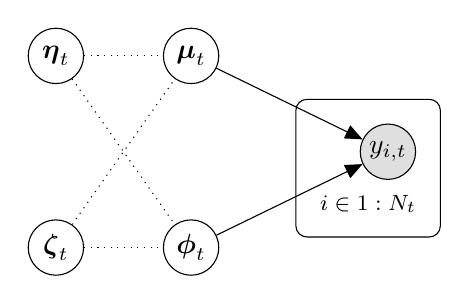
\begin{tikzpicture}
  % Define nodes
  \node[obs]                                     (y)  {$y_{i,t}$};
  \node[latent, above=0.5cm of y, xshift=-2.5cm] (mu)  {$\boldsymbol{\mu}_{t}$};
  \node[latent, below=0.5cm of y, xshift=-2.5cm] (phi)  {$\boldsymbol{\phi}_{t}$};
  \node[latent, left=1cm of mu]                   (eta) {$\boldsymbol{\eta}_t$};
  \node[latent, left=1cm of phi]                   (zeta) {$\boldsymbol{\zeta}_t$};

  % Connect the nodes with arrows for distributions
  \edge {mu,phi} {y} ; %

  % Connect the nodes with dotted lines for transformations
  \draw[dotted] (eta) -- (mu) ; %
  \draw[dotted] (zeta) -- (mu) ; %
  \draw[dotted] (eta) -- (phi) ; %
  \draw[dotted] (zeta) -- (phi) ; %

  % Plates
  \plate [inner sep = .3cm]{N} {(y)} {$i\in1:N_t$} ;

  \end{tikzpicture}
  \caption{A graphical representation of the B-spline beta regression model.}
  \label{fig:graphical_bsbr}
\end{figure}

Here, $\textit{t}$ relates to the training turbine, whilst $\textit{N}_t$ relates to the number of training data points for that turbine. In this initial case, independent models are learned per turbine \textit{t}, used to model the observed target variable $y_{i,t}$. $\mathbf{y}_t$, the column vector with entries \( y_{i,t} \) for \( i = 1, 2, \ldots, N_t \), is distributed according to the reparameterised Beta distribution,

\begin{equation} \label{eq:y}
  \mathbf{y}_t \sim \mathrm{Beta}(\boldsymbol{\mu}_{t},\boldsymbol{\phi}_{t})
\end{equation}

\noindent Additionally, hyperpriors were placed over the estimated parameters $\boldsymbol{\eta}_t$ and $\boldsymbol{\zeta}_t$, according to a Normal distribution,

\begin{equation} \label{eq:eta}
  \{\boldsymbol{\eta_t}, \boldsymbol{\zeta_t}\} \sim \mathcal{N}(0, 3) \quad \text{(element-wise)}
\end{equation}

\noindent where the means and standard deviations of 0 and 3 respectively were found to be weakly informative, while sufficiently aiding convergence.

\subsection{Inference}
The observed variables in graphical models may be referred to as evidence nodes~\cite{gelman2013bayesian}. In the example in Figure \ref{fig:graphical_bsbr}, the regression would have the following evidence nodes:

\begin{equation}
\mathcal{E}=\left\{\mathbf{y}_t\right\}
\end{equation}

\noindent Latent variables on the other hand are \textit{hidden} nodes,

\begin{equation}
\mathcal{H}=\left\{\boldsymbol{\eta}_t, \boldsymbol{\zeta}_t\right\}
\end{equation}

\noindent Bayesian inference relies on finding the posterior distribution of $\mathcal{H}$ given $\mathcal{E}$, that is, the distribution of the unknown parameters given the data,

\begin{equation}
  \begin{aligned}
    p(\mathcal{H} \mid \mathcal{E})=\frac{p(\mathcal{E} \mid \mathcal{H})p(\mathcal{H})}{p(\mathcal{E})}\\
    & = \frac{p(\mathbf{y_t} \mid \boldsymbol{\eta}_t, \boldsymbol{\zeta}_t) p(\boldsymbol{\eta}_t) p(\boldsymbol{\zeta}_t)}{p(\mathbf{y_t})}\\
    & = \frac{p(\mathbf{y_t} \mid \boldsymbol{\eta}_t, \boldsymbol{\zeta}_t) p(\boldsymbol{\eta}_t) p(\boldsymbol{\zeta}_t)}{\int\int p(\mathbf{y_t} \mid \boldsymbol{\eta}_t, \boldsymbol{\zeta}_t)p(\boldsymbol{\eta}_t) p(\boldsymbol{\zeta}_t) d\boldsymbol{\eta}_t d\boldsymbol{\zeta}_t}
  \end{aligned}
  \label{eq:bsbr_posterior}
\end{equation}

As is common in Bayesian inference problems, the integral in this case is intractable, and cannot be solved analytically. In this work, the posterior distribution is approximated using the Monte Carlo Markov Chain (MCMC) method, via the no U-turn (NUTS) implementation of Hamiltonian Monte Carlo (HMC)~\cite{homan_no-u-turn_2014}.  

\section{A Metamodelling Approach}\label{section:meta_model}

\subsection{Hierarchical Bayesian Modelling for Multi-task Learning}

In Section \ref{section:bsbr}, the presented BSBR model can be described as being an example of Single Task Learning (STL), since the task-level parameters $\boldsymbol{\eta}_t$ and $\boldsymbol{\zeta}_t$ are learned independently for each task; in this case, there is no-pooling (NP) of information between tasks. In contrast, a model containing parameters solely at the population-level which are shared across all tasks, can be said to have a complete-pooling (CP) modelling structure. In this case, all tasks are treated as identical, which can lead to poor model generalisation to new tasks. Alternatively, hierarchical Bayesian models (also known as multi-level models) provide a middle-ground, containing both task-specific parameters (allowing for differences between population members), and population-level parameters, which encourage task parameters to be similar; this modelling structure can be described as having partial-pooling (PP) of information. These models are often used as an approach to multi-task learning (MTL), where the goal is to improve the performance and generalisation of a model, by training it on multiple related tasks simultaneously~\cite{murphy2012machine}.

In the context of power-curve modelling, allowing PP of information makes intuitive sense; wind-turbines within a wind-farm are nominally identical, so they are likely to have similar power-curves (at a population-level), but differences may also arise from varying wake patterns at individual turbine locations (the task-level). An additional benefit of PP of information, is that data-poor tasks in particular are able to borrow statistical strength from data-rich tasks. Whilst in this context data availability is not a significant problem, it is commonly in the field of data-driven SHM~\cite{farrar_structural_2012}, which has led to these modelling approaches being used as a solution in the domain of Population-based SHM (PBSHM) research~\cite{bull_hierarchical_2022,dardeno_hierarchical_2024}.


\subsection{Metamodel Design}
In the results in Section \ref{section:bsbr_results}, correlations are observed among the learned $\boldsymbol{\eta}_t$ and $\boldsymbol{\zeta}_t$ parameters of the turbine-independent BSBR models, in relation to the turbine $x$ and $y$ spatial coordinates. This fact motivated the integration of a ``metamodel'', which can be described as a model over models. This metamodel was designed to capture the inter-turbine relationships in power-curve parameters, which could be used to predict power for previously unobserved turbines, not necessarily in the training data. This model design has a tangible real-world benefit - if one were able to make accurate probabilistic predictions for a variable of interest, at a location without data (and perhaps even without associated telemetry), this may reduce the overall telemetry requirements among a population. Whilst in the use case here data are readily available at each turbine location, it serves as a useful testbed to experiment with the modelling approach.

First-order linear metamodels were chosen here for both simplicity and to reduce the risk of overfitting to the training data. In matrix form, the parameter vectors $\boldsymbol{\eta}$ and $\boldsymbol{\zeta}$ are described via the linear metamodels,

\begin{equation}\label{eq:eta_meta}
  \boldsymbol{\eta} = \mathbf{C_x}\mathbf{M}_{\boldsymbol{\eta}_\mathbf{x}} + \mathbf{C_y}\mathbf{M}_{\boldsymbol{\eta}_\mathbf{y}}
\end{equation}

\begin{equation}\label{eq:zeta_meta}
  \boldsymbol{\zeta} = \mathbf{C_x}\mathbf{M}_{\boldsymbol{\zeta}_\mathbf{x}} + \mathbf{C_y}\mathbf{M}_{\boldsymbol{\zeta}_\mathbf{y}}
\end{equation}

\noindent where $\mathbf{C_x}$ and $\mathbf{C_y}$ are the linear regression design matrices for the normalised $x$ and $y$ coordinates for each turbine, and $\mathbf{M}_{\boldsymbol{\eta}_\mathbf{x}}$ and $\mathbf{M}_{\boldsymbol{\eta}_\mathbf{y}}$ are the metamodel parameter matrices for parameter vector $\boldsymbol{\eta}$. Similarly, $\mathbf{M}_{\boldsymbol{\zeta}_\mathbf{x}}$ and $\mathbf{M}_{\boldsymbol{\zeta}_\mathbf{y}}$ are the metamodel parameter matrices for parameter vector $\boldsymbol{\zeta}$.

As in the BSBR NP model, hyperpriors were used to aid model convergence, and were placed over the metamodel parameter matrices assuming normal distributions, 

\begin{equation}\label{eq:meta_priors}
  \{\mathbf{M}_{\boldsymbol{\eta}}, \mathbf{M}_{\boldsymbol{\zeta}}\} \sim \mathcal{N}(0, 3) \quad \text{(element-wise)}
\end{equation}

\noindent where $\mathbf{M}_{\boldsymbol{\eta}} = \left\{\mathbf{M}_{\boldsymbol{\eta}_\mathbf{x}},\mathbf{M}_{\boldsymbol{\eta}_\mathbf{y}}\right\}$ and $\mathbf{M}_{\boldsymbol{\zeta}} = \left\{\mathbf{M}_{\boldsymbol{\zeta}_\mathbf{x}},\mathbf{M}_{\boldsymbol{\zeta}_\mathbf{y}}\right\}$ and the prior means and standard deviations were we set equal to 0 and 3 respectively, given the distribution of learned parameters seen for the individual BSBR models; these were again found to be weakly informative, while sufficiently aiding convergence. Figure \ref{fig:graphical_meta} shows a graphical representation of the model. As with Figure \ref{fig:graphical_bsbr}, arrows represent distribution inputs, whilst dotted lines show calculated inputs, with plates indicating multiple instances of their contained nodes.

%% graphical model
\begin{figure}[H]
  \centering
  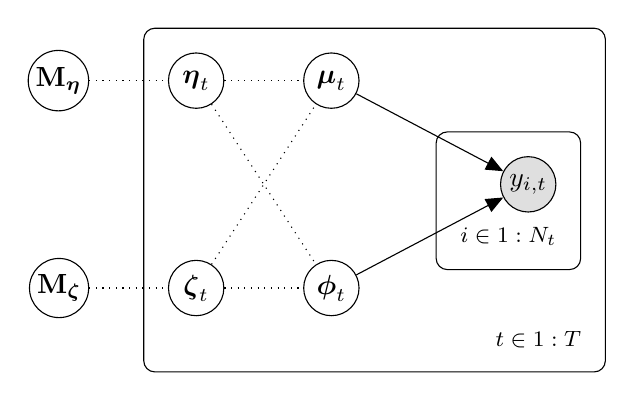
\begin{tikzpicture}
  % Define nodes
  \node[obs]                                     (y)  {$y_{i,t}$};
  \node[latent, above=0.6cm of y, xshift=-2.5cm] (mu)  {$\boldsymbol{\mu}_{t}$};
  \node[latent, below=0.6cm of y, xshift=-2.5cm] (phi)  {$\boldsymbol{\phi}_{t}$};
  \node[latent, left=1cm of mu]                   (eta) {$\boldsymbol{\eta}_t$};
  \node[latent, left=1cm of phi]                   (zeta) {$\boldsymbol{\zeta}_t$};
  \node[latent, left=1cm of eta] (meta_eta) {$\mathbf{M}_{\boldsymbol{\eta}}$};
  \node[latent, left=1cm of zeta] (meta_zeta) {$\mathbf{M}_{\boldsymbol{\zeta}}$};

  % Connect the nodes with dotted lines for calculations
  \draw[dotted] (meta_eta) -- (eta) ; %
  \draw[dotted] (meta_zeta) -- (zeta) ; %
  \draw[dotted] (eta) -- (mu) ; %
  \draw[dotted] (zeta) -- (mu) ; %
  \draw[dotted] (eta) -- (phi) ; %
  \draw[dotted] (zeta) -- (phi) ; %

  % Connect the nodes with arrows for distributions
  \edge {mu} {y} ;
  \edge {phi} {y} ;
  
  % Plates
  \plate [inner sep = .3cm]{N} {(y)} {$i\in1:N_t$} ;
  \plate [inner sep = .3cm]{T} {(y)(mu)(phi)(eta)(zeta)(N.north west)(N.south east)} {$t\in1:T$} ;

  \end{tikzpicture}
  \caption{A graphical representation of the metamodel. Arrows leading from parameters indicate they are distribution parameters, whereas dotted lines indicate parameters are associated via a transformation.}
  \label{fig:graphical_meta}
\end{figure}

\noindent Note that the metamodel parameters are located outside the plates, and are therefore learned at the population-level, whilst the parameters $\boldsymbol{\eta}_t$ and $\boldsymbol{\zeta}_t$ are learned specifically for each turbine. 

\subsection{Metamodel Predictions}

%\clearpage
% \FloatBarrier  % Ensures that all floats above are placed before proceeding

\begin{mdframed}
  Following posterior estimation of the population-level metamodel parameters, one can make probabilistic predictions at locations of interest based on spatial coordinates alone, 

  \begin{equation}\label{eq:meta_eta_pred}
    \boldsymbol{\eta^*} = \mathbf{C_x^*}\mathbf{\hat{M}}_{\boldsymbol{\eta}_\mathbf{x}} + \mathbf{C_y^*}\mathbf{\hat{M}}_{\boldsymbol{\eta}_\mathbf{y}}
  \end{equation}
  
  \begin{equation}\label{eq:meta_zeta_pred}
    \boldsymbol{\zeta^*} = \mathbf{C_x^*}\mathbf{\hat{M}}_{\boldsymbol{\zeta}_\mathbf{x}} + \mathbf{C_y^*}\mathbf{\hat{M}}_{\boldsymbol{\zeta}_\mathbf{y}}
  \end{equation}
\end{mdframed}

\noindent where $\boldsymbol{\eta^*}$ and $\boldsymbol{\zeta^*}$ are the predicted metamodel parameters for all turbine locations of interest, $\mathbf{{C_x}^*}$ and $\mathbf{{C_y}^*}$ are their associated first-order linear regression design matrices for the normalised spatial coordinates, and $\mathbf{\hat{M}}_{\boldsymbol{\eta}_\mathbf{x}}$, $\mathbf{\hat{M}}_{\boldsymbol{\eta}_\mathbf{y}}$, $\mathbf{\hat{M}}_{\boldsymbol{\zeta}_\mathbf{x}}$ and $\mathbf{\hat{M}}_{\boldsymbol{\zeta}_\mathbf{y}}$ are the estimated metamodel parameters. The predicted parameters can then be used in line with the population-level input features (and associated \textit{Q} matrix) to make probabilistic power-predictions.


\subsection{Metamodel Benchmarking}
The model presented in Section \ref{section:meta_model} represents a hierarchical Bayesian model (with \textit{partial-pooling}), incorporating a metamodel---this complete model is simply referred to as the metamodel. To help assess the performance of the metamodel, it is benchmarked against three models which do not account for spatial correlation between turbines. The first of these, is the basic BSBR model shown in Figure \ref{fig:graphical_bsbr}, which as compared to the metamodel, has no-pooling nor any linear model constraints between turbine-specific parameters. Secondly the metamodel is compared to a similarly partially-pooled hierarchical model (shown in Figure \ref{fig:pp_model}), but where the population-level parameters more simply describe the population mean and standard deviation of the turbine-specific parameters, thus not imposing a linear model constraint over them; this should help test the suitability of the linear metamodel assumption over the turbine-specific parameters. For completeness, the metamodel is compared to a complete-pooling approach, where all turbines are considered identical and a single set of model parameters is learned for all turbines; this is shown in Figure {\ref{fig:cp_model}}. For further details, \texttt{stan} code containing the four models is provided in the links in Section \ref{section:data_availability}.

%%%%%%%%%%%%%%%%%%%%%%
%%% Partial Pooling %%%
%%%%%%%%%%%%%%%%%%%%%%
\begin{figure}[h]
  \centering
  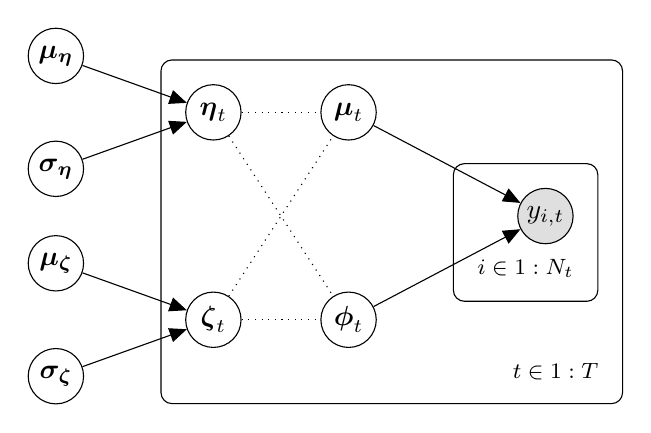
\begin{tikzpicture}
  % Define nodes
  \node[obs]                                     (y)  {$y_{i,t}$};
  \node[latent, above=0.6cm of y, xshift=-2.5cm] (mu)  {$\boldsymbol{\mu}_{t}$};
  \node[latent, below=0.6cm of y, xshift=-2.5cm] (phi)  {$\boldsymbol{\phi}_{t}$};
  \node[latent, left=1cm of mu]                   (eta) {$\boldsymbol{\eta}_t$};
  \node[latent, left=1cm of phi]                   (zeta) {$\boldsymbol{\zeta}_t$};
  \node[latent, above=0cm of eta, xshift=-2cm] (mu_eta) {$\boldsymbol{\mu_{{\eta}}}$};
  \node[latent, below=0cm of eta, xshift=-2cm] (sig_eta) {$\boldsymbol{\sigma_{{\eta}}}$};
  \node[latent, above=0cm of zeta, xshift=-2cm] (mu_zeta) {$\boldsymbol{\mu_{{\zeta}}}$};
  \node[latent, below=0cm of zeta, xshift=-2cm] (sig_zeta) {$\boldsymbol{\sigma_{{\zeta}}}$};


  % priors

  % Connect the nodes with dotted lines for calculations
  \draw[dotted] (eta) -- (mu) ; %
  \draw[dotted] (zeta) -- (mu) ; %
  \draw[dotted] (eta) -- (phi) ; %
  \draw[dotted] (zeta) -- (phi) ; %

  \edge {mu_eta} {eta} ; %
  \edge {sig_eta} {eta} ; %
  \edge {mu_zeta} {zeta} ; %
  \edge {sig_zeta} {zeta} ; %

  \edge {mu} {y} ;
  \edge {phi} {y} ;
  
  % Plates
  \plate [inner sep = .3cm]{N} {(y)} {$i\in1:N_t$} ;
  \plate [inner sep = .3cm]{T} {(y)(mu)(phi)(eta)(zeta)(N.north west)(N.south east)} {$t\in1:T$} ;

  \end{tikzpicture}
  \caption{Partially-pooled (PP) BSBR graphical model.}
  \label{fig:pp_model}
\end{figure}

%%%%%%%%%%%%%%%%%%%%%%
%%% Complete Pooling %%%
%%%%%%%%%%%%%%%%%%%%%%
\begin{figure}[h]
  \centering
  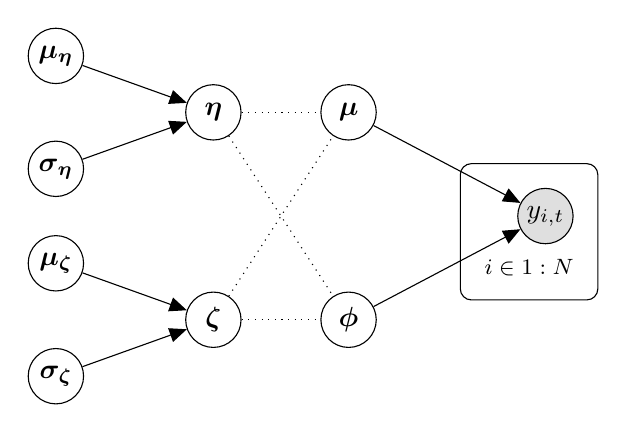
\begin{tikzpicture}
  % Define nodes
  \node[obs]                                     (y)  {$y_{i,t}$};
  \node[latent, above=0.6cm of y, xshift=-2.5cm] (mu)  {$\boldsymbol{\mu}$};
  \node[latent, below=0.6cm of y, xshift=-2.5cm] (phi)  {$\boldsymbol{\phi}$};
  \node[latent, left=1cm of mu]                   (eta) {$\boldsymbol{\eta}$};
  \node[latent, left=1cm of phi]                   (zeta) {$\boldsymbol{\zeta}$};
  \node[latent, above=0cm of eta, xshift=-2cm] (mu_eta) {$\boldsymbol{\mu_{{\eta}}}$};
  \node[latent, below=0cm of eta, xshift=-2cm] (sig_eta) {$\boldsymbol{\sigma_{{\eta}}}$};
  \node[latent, above=0cm of zeta, xshift=-2cm] (mu_zeta) {$\boldsymbol{\mu_{{\zeta}}}$};
  \node[latent, below=0cm of zeta, xshift=-2cm] (sig_zeta) {$\boldsymbol{\sigma_{{\zeta}}}$};


  % priors

  % Connect the nodes with dotted lines for calculations
  \draw[dotted] (eta) -- (mu) ; %
  \draw[dotted] (zeta) -- (mu) ; %
  \draw[dotted] (eta) -- (phi) ; %
  \draw[dotted] (zeta) -- (phi) ; %

  \edge {mu_eta} {eta} ; %
  \edge {sig_eta} {eta} ; %
  \edge {mu_zeta} {zeta} ; %
  \edge {sig_zeta} {zeta} ; %

  \edge {mu} {y} ;
  \edge {phi} {y} ;
  
  % Plates
  \plate [inner sep = .3cm]{N} {(y)} {$i\in1:N$} ;

  \end{tikzpicture}
  \caption{Completely-pooled (CP) BSBR graphical model.}
  \label{fig:cp_model}
\end{figure}


%%%%%%%%%%%%%%%%%%%%%%%%%%%%%%%%%%%
% Model setup
%%%%%%%%%%%%%%%%%%%%%%%%%%%%%%%%%%%

\section{Model Training and Testing}\label{section:model_training}

\subsection{Training and Testing Datasets}\label{section:traintest}

\subsubsection{BSBR Model Demonstration}
In the first instance, to demonstrate the suitability of the BSBR model for capturing the heteroscedastic and asymmetric nature of power-curves, the model is trained and tested on individual turbines (i.e.\ using the no-pooling model definition). A subset of the filtered data that had undergone stratified sampling by yaw angle is used, to provide the models with an approximately even distribution of data across yaw angles, to try to help make the models more generalisable to all wind directions. The training and testing datasets consisted of 4000 and 1000 data points per turbine respectively.

\subsubsection{Metamodel}
In the SCADA data, it was noted that there were significant proportions at zero or maximum power; because of this, additional stratified sampling was applied based on measured turbine output power. The reasons for doing this were twofold: (1) to train and assess models equally for all regions of the power-curve (2) because of the heteroscedastic nature of the power-curve, harmonising the proportions of data in different regions of the power-curve between turbines was considered to make comparisons between predictive metrics more reasonable. Since the metamodel aims to capture spatial correlations induced by wake effects, reason (1) is particularly important, since wake effects are more prevalent in the transitional region of the power-curve \cite{howland_wind_2019}, which is comparatively data-sparse.

Additionally, for the metamodel, since a single model is learned for all data simultaneously, because of increased computational expense a reduced number of training points were needed. The resulting training and testing sets, having undergone stratified sampling on both the yaw angle and output power, consisted of just 250 points per turbine, which were used for the metamodel and benchmark models. Furthermore, since the metamodel and benchmark models are to be trained on a subset of the turbines, as an example 1/4 of the turbines were used, approximately equally spaced throughout the wind-farm. The training and testing turbines are highlighted in Figure \ref{fig:train_test_map}. The resulting combined training and test sets consisted of 5000 and 20000 data points respectively.

\begin{figure}[h]
  \centering
    \includegraphics[width=\textwidth]{figures/final/train_test_map.png}
    \caption{Map showing the training and testing turbines for the metamodel. Red circles show the locations of the turbines used in training, while all turbines (shown in blue) were used in testing.}
    \label{fig:train_test_map}
  \end{figure}

\subsection{Model Training}\label{sec:model_training}

As previously discussed, MCMC is used to estimate the posterior distributions of our parameters, given observed levels of power per turbine. MCMC was implemented using \texttt{stan} \cite{stan_development_team_stan_2024}, with 2000 burn-in and 2000 inference samples per chain, and four chains. As discussed in the methods, to aid computational efficiency we use the QR decomposition on the design matrix as recommended in the \texttt{stan} users guide~\cite{stan_development_team_stan_2024}. For the full details of the \texttt{stan} models, please see the code available at: \url{https://github.com/smbrealy/wind_mtl}. 

\subsection{Model Scoring}\label{section:scoring}
In order to quantify the success of each of the models, two performance metrics were used. Firstly, the Normalised Mean Squared Error (NMSE) assesses the goodness-of-fit, or how close point predictions are to their test value. The NMSE functions similarly to percentage error, where a score of zero indicates a perfect model, whilst a score of 100 is equivalent to a model simply predicting the mean value of the data. NMSE is defined as,

\begin{equation}\label{eq:NMSE}
  \mathrm{NMSE}=\frac{100}{N \sigma_y^2} \sqrt{(\mathbf{y}-\widehat{\mathbf{y}}){^\intercal}(\mathbf{y}-\widehat{\mathbf{y}})}
\end{equation}
\noindent where $N$ is the number of data points, $\sigma_y^2$ is the variance of the measured data, $\mathbf{y}$ the measured data, and $\widehat{\mathbf{y}}$ the model predictions. 

Since the models are probabilistic and include predictive variance, the joint-log-likelihood (JLL) is also calculated as a measure of how well the uncertainty in the measured data was captured by the model, which NMSE does not. The JLL is calculated as,

\begin{equation}\label{eq:JLL}
  JLL=\frac{\sum_{s=1}^{S}\sum_{i=1}^{N_t}\log{f(y_{{i,t}_s}|{\mu}_{{i,t}_s}, {\phi}_{{i,t}_s})}}{S}
\end{equation}

\noindent where $f(y_{{i,t}_s}|{\mu}_{{i,t}_s}, {\phi}_{{i,t}_s})$ is the probability density function of the beta distribution as defined in equation (\ref{eq:beta_dist}), and \textit{S} is the number of posterior samples. The larger the JLL, the better the model has captured the true distribution of the test data. Given the prevalence of power-curve modelling in the literature, it's worth stating that since the model metrics are dependant upon both the training features and test data used, they are best used as a comparison of the models within this paper only.

%%%%%%%%%%%%%%%%%%%%%%%%%%%%%%%%%%%
% Results
%%%%%%%%%%%%%%%%%%%%%%%%%%%%%%%%%%%

\section{Results and Discussion}\label{section:results}

\subsection{BSBR Model Demonstration}\label{section:bsbr_results}

To first demonstrate probabilistic predictions that can be made with the BSBR models (with no-pooling), Figure \ref{fig:BSBR model predictions} shows predictions from models of turbines on both the west and east-side of the wind-farm in subplots (a) and (b) respectively. Test data are indicated by red crosses, model mean predictions are indicated by circles (which are coloured by the value of the wind direction), and model uncertainty is represented by the blue shaded area--indicating the 95$^{th}$-percentile uncertainty bounds.

\begin{figure}[h!]
  \centering
  \begin{subfigure}{0.7\textwidth}
   % \centering
    \includegraphics[width=\textwidth]{figures/final/west_side_turbine.png}
    \caption{West-side turbine.}
    \label{fig:west_side}
  \end{subfigure}%

  \bigskip
  \begin{subfigure}{0.7\textwidth}
    %\centering
    \includegraphics[width=\textwidth]{figures/final/east_side_turbine.png}
    \caption{East-side turbine.}
    \label{fig:east_side}
  \end{subfigure}
  \caption{BSBR NP model predictions for two separate turbines. Test data are shown by red crosses, mean predictions are shown as circles, coloured by the wind direction. The blue shaded areas show the 95$^{th}$-percentile of the predictive variance.}
  \label{fig:BSBR model predictions}
  \end{figure}


There are a number of interesting observations. Firstly, the predictive uncertainty appears to match the data, with reduced variance at the lower and upper ends of the curve, and increased variance in the transitional region between turbine minimum and maximum power. Approximately 5\% of the test points also lie outside the 95$^{th}$-percentile of the predictive variance, as should be expected for a correctly-trained model. The ``rough'' edges of this uncertainty are from data points that, while having a very similar freestream wind speed, may have significantly different wind directions, which also contribute to the predictive uncertainty. Secondly, while the majority of the influence on output power appears to be associated with the freestream wind speed (as expected), the models have allocated some weight to the wind-directional features, resulting in the variance in the mean predictions for a given freestream wind speed; this is mostly prevalent in the transitional region between minimum and maximum power, and matches intuition since turbine wakes affect this region the most. However, in this region it is clear that significant deviation between model mean predictions and the test data remains. This deviation is likely the result of a number of factors, including the oversimplification of the wake effect by assuming it can be approximated based on the wind direction. In reality, this fails to account for atmospheric conditions such as wind shear, turbulence intensity, thermal stratification and air-density variations, which are known to have an impact on wake propagation~\cite{nielson_using_2020,barthelmie_evaluation_2010}. Furthermore, in calculating the input features, the wind direction (yaw angle) is assumed to be the same for all turbines - this is not the case, as there is a distribution of localised wind-directions across the wind-farm (yaw angles), which will likely change the wake patterns. There are also additional sources of noise within the data, such as sensor calibration errors in the yaw and wind speed measurements which are used in calculating the population-level features, as well as possible changes in the underlying behaviour of the turbines, perhaps because of wear or damage during the period of the training data used. Additionally, \textit{curtailed}, \textit{shut-down} or even \textit{power-boosted} turbines upstream of a given turbine will further generate noise in the wake patterns.

Despite these problems, comparison of the west and east-side models yields some evidence that a level of turbine-dependent wind-directionality has been captured. For example, for the west-side turbine, it is not expected to be influenced by wakes when wind approaches from the western direction (equivalent to a value of 0 for feature two). Conversely, the east-side turbine is not expected to be influenced by wakes when wind blows from the east (equivalent to a value of 1 for feature three). In each case, the models appear to predict higher levels of power when these conditions are true, and less power when they are not, as one would expect to be the case in reality. While not shown here, these characteristics can also be seen for other turbine models around the perimeter of the wind-farm, to similar or lesser degrees.

To explore this model behaviour further, the learned model parameter vectors which result in differences in predicted values may be inspected. In this case, each of the vectors $\boldsymbol{\eta}$ and $\boldsymbol{\zeta}$ consist of 18 parameters, with parameters 1-6 associated with Feature One, 7-12 Feature Two and 13-18 Feature Three. Figure \ref{fig:weightcorrelations} shows the value of selected parameters from the $\boldsymbol{\eta}$ vector plotted for each turbine within the wind-farm. The colour of the points denotes the values of the parameters as indicated by the colour bars. 

For Parameter Four (associated with Feature One), there does not appear to be an obvious spatial correlation. However, while their magnitude is considerably smaller than Parameter Four, Parameters Eight and 13 (associated with Features Two and Three), shown in subfigures \ref{fig:weight_8} and \ref{fig:weight_13}, show clear spatial correlation across the wind-farm. For Parameter Eight, there is an approximate negative correlation from west to east, whilst there is an approximate south to north negative correlation for Parameter 13. While not shown here, similar observations can be made for the remaining parameters in the $\boldsymbol{\eta}$ and $\boldsymbol{\zeta}$ vectors. These spatial differences in parameters represent the wake effect captured by the NP models, and motivated the development of the metamodel, which aims to remove the requirement for data from each turbine location, by utilising the correlation in parameters. The use of a partially-pooled hierarchical model in this case also allows ``statistical strength'' to be shared between turbine-specific parameters, via the population-level parameters.
\begin{figure}[H]
  \begin{subfigure}{\textwidth}
    \centering
    \includegraphics[width=.7\textwidth]{figures/final/np_eta_param_4_v2.png}
    \caption{4th parameter in the learned $\boldsymbol{\eta}$ vectors.}
    \label{fig:weight_4}
  \end{subfigure}

\end{figure}
  \begin{figure}[H]\ContinuedFloat
  \begin{subfigure}{\textwidth}
    \centering
    \includegraphics[width=.7\textwidth]{figures/final/np_eta_param_8_v2.png}
    \caption{8th parameter in the learned $\boldsymbol{\eta}$ vectors.}
    \label{fig:weight_8}
  \end{subfigure}

\end{figure}
\begin{figure}[H]\ContinuedFloat
  \begin{subfigure}{\textwidth}
    \centering
    \includegraphics[width=0.7\textwidth]{figures/final/np_eta_param_13_v2.png}
    \caption{13th parameter in the learned $\boldsymbol{\eta}$ vectors.}
    \label{fig:weight_13}
  \end{subfigure}
  \caption{Mean parameter values of selected entries of the learned BSBR model $\boldsymbol{\eta}$ vectors, plotted by turbine location. Colours indicate the value of the parameters.}
  \label{fig:weightcorrelations}
  \end{figure}


\subsection{Metamodel}

The metamodel learns linear models over the parameter vectors, for turbine $x$ and $y$ coordinates. The right-hand plots in sub-Figures \ref{fig:weight4comparison} and \ref{fig:weight8comparison} show the metamodel mean predicted value by colour, plotted spatially, for $\boldsymbol{\eta}$ Parameters Four and Eight respectively. Filled circles denote the locations of the turbines used for training the metamodel, whilst unfilled circles represent the locations of the remaining unobserved turbines used in testing. These predictions are compared directly with the NP BSBR models, shown in the left-hand plots. As with Figure \ref{fig:weight_4}, there is limited spatial correlation for Parameter Four seen for the NP model, which for the metamodel resulted in very little spatial difference in this parameter across all turbines. In contrast, for Parameter Eight it can be seen that the metamodel has learned the more significant correlation seen in the NP model parameters. These observations could suggest that the linear model assumption offers a level of regularisation, and is able to capture intuitively the general observable spatial correlation in parameters. 

\begin{figure}[H]
  \centering
  \begin{subfigure}{\textwidth}
    \centering
    \includegraphics[width=\textwidth]{figures/final/eta_4_comparison_v2.png}
    \caption{4th parameter in the learned $\boldsymbol{\eta}$ vectors.}
    \label{fig:weight4comparison}
  \end{subfigure}
\end{figure}
\begin{figure}[H]\ContinuedFloat
  \begin{subfigure}{\textwidth}
    \centering
    \includegraphics[width=\textwidth]{figures/final/eta_8_comparison_v2.png}
    \caption{8th parameter in the learned $\boldsymbol{\eta}$ vectors.}
    \label{fig:weight8comparison}
  \end{subfigure}
  \caption{Mean predicted values for the fourth (subplot (a)) and eighth (subplot (b)) entries in the $\boldsymbol{\eta}$ parameter vector, plotted spatially for each turbine in wind-farm \textit{Ciabatta}. In each subplot, the left-hand plots show predictions from the NP model, whilst the right-hand plots show metamodel predictions. Filled circles represent turbines used in training, whilst unfilled circles represent turbines used in testing only. The colours of the points represent the values of the parameters.}
  \label{fig:metacorrelations}
\end{figure}


\subsubsection{Model Scores}

The metamodel is compared against the benchmark NP, PP and CP models, using the scoring metrics. Figure \ref{fig:NMSE} shows the NMSE per turbine, for each model, with a lower score indicating an improved performance on the turbine's associated test data. Figure \ref{fig:JLL} shows the JLL per turbine, for each model, with a higher score indicating an improved performance on the turbine's associated test data. In both figures, the vertical dashed lines denote turbines used in training.
\begin{figure}[h]

  \begin{subfigure}{\textwidth}
  \includegraphics[width=\textwidth]{figures/final/NMSE_2000_v2.png}
  \caption{NMSE scores}
  \label{fig:NMSE}
  \end{subfigure}
  
  \bigskip
  
  \begin{subfigure}{\textwidth}
  \includegraphics[width=\textwidth]{figures/final/JLL_2000_v2.png}
  \caption{JLL scores}
  \label{fig:JLL}
  \end{subfigure}

  \caption{Comparison of model scores for each turbine in wind-farm \textit{Ciabatta}. For the metamodel, CP and PP models, the vertical dashed lines denote turbines used in training. Coloured dashed horizontal lines represent the mean score across all turbines for each model.}
  \label{fig:scores}
\end{figure}

For both metrics, it can be seen that the CP model performs significantly worse than the other models, which perform more similarly to each another; this suggests a benefit in accounting for task-level differences, which the CP model does not. There are some instances however where the NP models perform worse the CP model on JLL, in particular for Turbines 17 and 58. During MCMC sampling, on some occasions a few of the NP model estimations resulted in divergences, which suggests the sampler was having difficulties exploring the posterior geometry; this was not the case for the other models, which may suggest that their sharing of information was helpful in parameter estimation \cite{gelman2013bayesian}.

More broadly, it can be seen on average that the PP model performs similarly but marginally better than the NP model, however the metamodel shows a more distinct improvement on both metrics, showing an average improvement of approximately 2.3\% in NMSE and 60 in JLL compared to the PP model. Moreover, the metamodel nearly always scores the highest on both metrics across all turbines, (including the previously-unobserved testing turbines); this provides validation that the assumptions used in the construction of the metamodel provide valuable information in the spatial prediction of wind-turbine power.

A final observation is that there are relatively-high NMSE scores across all models for Turbines 40--50 (and relatively low JLL), followed by lower scores of Turbines 50--60; to explore this further, the scoring metrics for the metamodel are plotted spatially in Figure \ref{fig:score_maps}. Here, in general the scores appear to be worse towards the lower end of the wind-farm; this matches intuition, since these turbines also follow a less rigid spatial pattern than the turbines at the upper end, which is likely to add additional noise to the spatial wake patterns of these turbines.

\begin{figure}[h]
  \centering
    \centering
    \includegraphics[width=\linewidth]{figures/final/NMSE_JLL_map.png} % Add your image path
    \caption{Maps of model scores across the wind farm. The left-hand plot shows the NMSE per turbine, whilst the right-hand plot shows the JLL per turbine.}
    \label{fig:score_maps}
\end{figure}

\subsubsection{Predicting Unobserved Turbines}
The models are now compared in prediction, for an unobserved turbine i.e.\ a turbine that was not used in training for the metamodel, PP and CP models. Figures \ref{fig:f1_a}--\ref{fig:f2_b} compare the learned linear models $f_1$ and $f_2$ across all four models. A gridded input over all three features was used, taking averages of the predictive mean and variance over the wind-directional Features Two and Three. Model mean predictions are shown as solid lines, while the shaded areas represent the $95^{th}$-percentile uncertainties. For the CP model, the predictive variance is relatively high for all values; which is reflective of the model not accounting for task-specific differences, and capturing the variance of all tasks in the learned parameters. The NP model also has relatively high predictive variance, particularly at the ends of the feature space where training data become more scarce; on the other hand, the PP and metamodels benefit from the sharing of statistical strength between turbines, and have reduced predictive variance across the feature space as a result, despite this turbine being unobserved.

\begin{figure}[htbp]
  \centering
  \begin{subfigure}{.45\textwidth}
    \centering
    \includegraphics[width=\linewidth]{figures/final/f1_a_2000_v2.png} % Add your image path
    \caption{$f_1$: metamodel and PP model}
    \label{fig:f1_a}
  \end{subfigure}
  \begin{subfigure}{.45\textwidth}
    \centering
    \includegraphics[width=\linewidth]{figures/final/f1_b_2000_v2.png} % Add your image path
    \caption{$f_1$: CP and NP model}
    \label{fig:f1_b}
  \end{subfigure}
  \begin{subfigure}{.45\textwidth}
    \centering
    \includegraphics[width=\linewidth]{figures/final/f2_a_2000_v2.png} % Add your image path
    \caption{$f_2$: metamodel and PP model}
    \label{fig:f2_a}
  \end{subfigure}
  \begin{subfigure}{.45\textwidth}
    \centering
    \includegraphics[width=\linewidth]{figures/final/f2_b_2000_v2.png} % Add your image path
    \caption{$f_2$: CP and NP model}
    \label{fig:f2_b}
  \end{subfigure}
  \caption{Posterior predictive distributions for functions $f_1$ and $f_2$, for turbine 35, using a gridded input over all three features. Averages were taken over Features Two and Three. Solid lines represent the mean prediction, while shaded areas show the $95^{th}$-percentile uncertainty.}
  \label{fig:f_functions}
\end{figure}

These observations carry into the full probabilistic power-predictions, as shown in Figure \ref{fig:unseen_preds}. Whilst a typical power-curve is ``sigmoidal'' in shape, in this case the shape of the model predictions differ slightly at higher freestream wind speeds, as a result of the stratified sampling carried out on the training and test data; this results in relative data sparsity at maximum power, particularly beyond a freestream wind speed of 0.8. For the NP model, this sparsity results in relatively high predictive variance in this region, with the model mean prediction also being partially ``dragged down'' towards zero - the default behaviour of B-spline models with no data. On the other hand, the metamodel and PP models benefit from the sharing of statistical strength between model parameters, resulting in reduced predictive variance; this demonstrates the advantage of the hierarchical modelling approach, although it does come with the cost of additional computational expense.

\begin{figure}[htbp]
  \centering
  \begin{subfigure}{.45\textwidth}
    \centering
        \includegraphics[width=\linewidth]{figures/final/preds_all_a_2000_v2.png} % Add your image path
        \caption{Metamodel and PP model.}
        \label{fig:preds_a}
  \end{subfigure}
  \begin{subfigure}{.45\textwidth}
    \centering
        \includegraphics[width=\linewidth]{figures/final/preds_all_b_2000_v2.png} % Add your image path
        \caption{CP and NP model.}
        \label{fig:preds_b}
  \end{subfigure}

  \caption{Probabilistic power-predictions on the ``unobserved'' turbine 35, over the gridded input data.}
  \label{fig:unseen_preds}
\end{figure}


%%%%%%%%%%%%%%%%%%%%%%%%%%%%%%%%%%%
% Conclusions
%%%%%%%%%%%%%%%%%%%%%%%%%%%%%%%%%%%

\section{Conclusions}\label{section:conclusions}

A probabilistic, multivariate wind-turbine power-prediction model was developed, utilising a beta regression model with B-spline basis functions (named the BSBR model). This BSBR model was shown to be successful in capturing both the heteroscedastic and asymmetric properties of power-curve data. When training the BSBR model on each turbine within a wind-farm, correlations were observed in the learned model parameters with respect to turbine locations, which were deemed to be associated with the directional dependency of turbine wakes. 

These spatial correlations in parameters were then leveraged via a ``metamodel'', which imposed functional constraints over turbine-specific parameters, as part of a partially-pooled hierarchical Bayesian model. This model design is able to learn from all turbines (tasks) simultaneously, and via the metamodel parameters, can be used to make adaptive probabilistic predictions for turbines not necessarily included in the training data, using their spatial coordinates alone. The metamodel was found to outperform three benchmark models that utilised no-pooling, partial-pooling and complete-pooling of information, both in terms of normalised mean squared error, and joint log-likelihood.

While for power-curve prediction, training data are readily available for all turbines, the results suggest that the metamodel design is an efficient modelling solution for situations where data may be limited, and correlations could be expected in a variable of interest among a population of structures. Potential further applications in this domain include (but are not limited to): structural load assessment for fatigue-life estimation, condition monitoring and fault detection, and design for wind-farm layouts.

A number of simplifying assumptions were made in relation to the training features to help capture wake effects from the data; these features may be improved if meteorological mast data were available, which would likely be a more accurate reflection of freestream wind conditions. Given the complexity of turbine wake physics, future work could also consider using physics-based inputs, to develop a hybrid data and physics based approach. Datasets labelled with turbine operating regimes, and instances of damage or repair that may indicate a change in underlying turbine behaviour, may also help with data preprocessing to reduce possible sources of noise. Model design may also be improved via optimisation of the number of B-spline knots per feature, their locations, or alternative spline-modelling approaches. The use of nonlinear metamodels may also worth considering, particularly if parameter spatial correlations are complex.

\section{Data availability}\label{section:data_availability}
For the purpose of reproducibility, the \texttt{stan} code used in this work has been made available online at: \url{https://github.com/smbrealy/wind_mtl}. The data used are part of a Non Disclosure Agreement and cannot be shared.

\section{Acknowledgements}
The authors gratefully acknowledge the support of the UK Engineering and Physical Sciences Research Council (EPSRC) and the Natural Environment Research Council (NERC), via grant references EP/W005816/1, EP/R003645/1 and EP/S023763/1. The authors also gratefully acknowledge Vattenfall R\&D for their time and for providing access to the data used in this study. For the purpose of open access, the author(s) has/have applied a Creative Commons Attribution (CC BY) licence to any Author Accepted Manuscript version arising.

% %% The Appendices part is started with the command \appendix;z
% %% appendix sections are then done as normal sections

% \appendix
% \section{Graphical Models}
% \label{sec:appendix}

%% If you have bibdatabase file and want bibtex to generate the
%% bibitems, please use
%%
\bibliographystyle{elsarticle-num-names} 
\bibliography{cas-refs}

%% else use the following coding to input the bibitems directly in the
%% TeX file.

% \begin{thebibliography}{00}

% %% \bibitem[Author(year)]{label}
% %% Text of bibliographic item

% \bibitem[ ()]{}

% \end{thebibliography}
\end{document}

\endinput
%%
%% End of file `elsarticle-template-num-names.tex'.
